%!TEX root = main.tex

\subsection{Dataset}

We  used NIST Special Database 4 \cite{nist-db-4} and NIST Special Database 14 \cite{nist-db-14} for our experiments. 

NIST SD4 contains $2000$ 8-bit gray scale fingerprint image pairs, a total of $4000$ images.  Each fingerprint pair consists of two different rollings of the same finger.
%
The size of each image is $512\times512$ pixels and each image is classified using one of the five following classes: Arch, Left or Right loops, Tented Arch, or Whorl.
%
The database is evenly distributed over each of the five mentioned classifications with $400$ fingerprint pairs ($800$ images) from each class. 

NIST SD14 contains $27000$ 8-bit gray scale fingerprint image pairs, a total of $54000$ images. There are 2700 subjects in this dataset and each subject has 10 fingerprint  pairs. The size of each image is  $768\times832$.  To fit in our network (see Section \ref{sec_cnn}), we centrally crop each image into a $768\times768$ pixels image and then resize it into $512\times512$ pixels using bilinear interpolation.
%
Each image is classified using the five finger pattern types mentioned above by professional fingerprint examiners.  Table \ref{tab.sd14_dist} shows the distribution of fingerprint pattern classes. The distribution of classes are supposed to approximate the natural horizontal distribution of the five pattern type classes.  We can see that unlike NIST SD4, arch and tented arch samples are only a small portion of NIST SD14.


\begin{table}[!ht]
	\centering
	\caption{Fingerprint Pattern Class Distribution of NIST SD14.}
\label{tab.sd14_dist}
	\begin{tabular}{|c|c|c|c|c|}
		\hline
		\textbf{Arch} & \textbf{Left Loop} & \textbf{Right Loop} & \textbf{\begin{tabular}[c]{@{}c@{}}Tented \\ Arch\end{tabular}} & \textbf{Whorl} \\ \hline
		3.6\% & 31.9\% & 30.5\% & 3.2\% & 30.8\% \\ \hline
	\end{tabular}
\end{table}

\subsection{Experimental Setup}
We used a i7-5930K desktop with 32GB memory and a Nvidia GTX TITAN X GPU for experiments.
%
We used Tensorflow 1.0.1 as the deep learning library and Adaptive Moment Estimation(Adam\cite{kingma2014adam}) as the optimization algorithm. The learning rate is 0.0001. We also used $\ell_2$ regularization with 0.0001 weight decay rate. The batch size is 32. 
%
We ran two sets of experiments using NIST SD4 and NIST SD14.  Each experiment is trained for $20k$ steps.

For the NIST SD14 experiment, we used images of the $80\%$ of the subjects for training, a total of $2160$ subjects, $43200$ images. Among these $432000$ images, $36$ of them have labels other than the 5 classes mentioned above. These $36$ images were discarded. 
Images from the remaining $20\%$ of the subjects are used for testing, a total of $10800$ images. $9$ of these images were discarded due to the same reason above.
%

For the NIST SD4 experiment, we adopted two evaluation protocols.
%
The first protocol is cross-sample, where we used the first samples of each fingerprint pair for training and the second samples for testing.  This is the same protocol used by previous works reported in the literature, and therefore allows for a more relevant comparison of our results with related works.
The second protocol is cross-finger, where we used images of 50\% of the fingers for training and the other 50\% for testing. This ensures images of the same finger does not exist in the training and testing sets at the same time. To improve the performance for the NIST SD4, we used NIST SD14 data to train the model, that is, the training data comprises of 50\% of NIST SD 4 and 100\% of NIST SD 14 images.
 
The following sections, report classification accuracy for 5-class fingerprint pattern type classification for two cases: a) SVM is trained as a classifier using deep features generated by our trained ConvNet, and b) ConvNet is used as the classifier.
Additionally, we evaluated the performance of the SVM on 4-class fingerprint classification where arch and tented arch classes are combined. 4-class classification is also reported in other studies.  
%
%To achieve 4-class classification, we merge Tented Arch class into Arch class when training SVM.

\begin{figure*}[!ht]
	\begin{subfigure}[b]{0.25\textwidth}
		\centering
		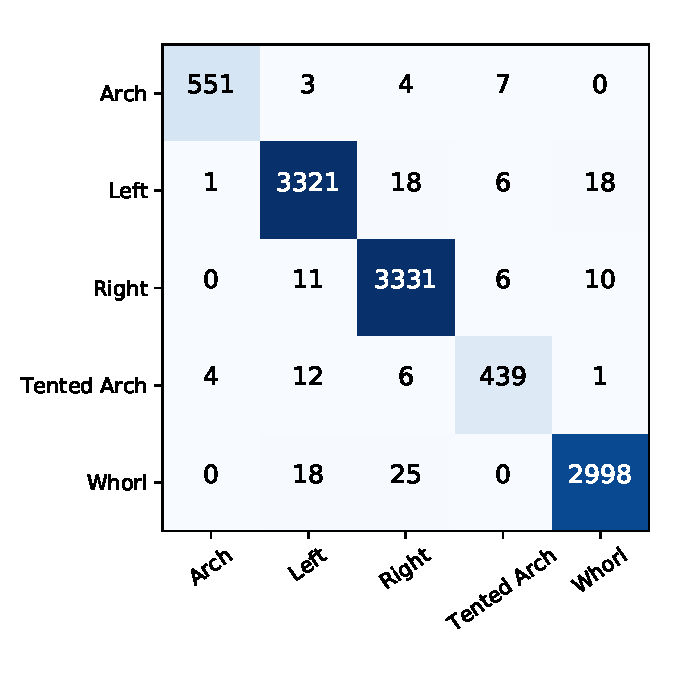
\includegraphics[width=\linewidth]{fig/figs/confusion_matrix_svm_sd14.pdf}
		\caption{SVM -- NIST SD14 }
		\label{fig.cnf_matrix_5class.svm_sd14}
	\end{subfigure}%
	\begin{subfigure}[b]{0.25\textwidth}
		\centering
		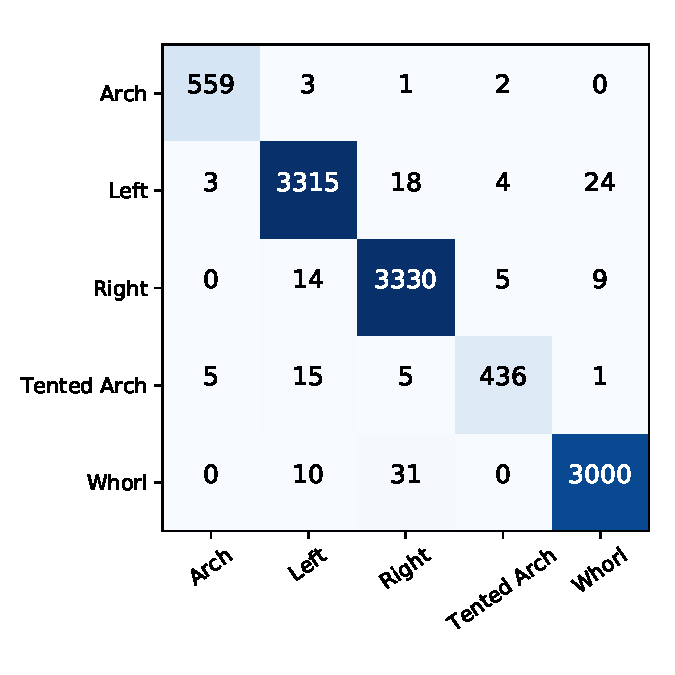
\includegraphics[width=\linewidth]{fig/figs/confusion_matrix_net_sd14.pdf}
		\caption{ConvNet -- NIST SD14 }
		\label{fig.cnf_matrix_5class.net_sd14}
	\end{subfigure}%
	\begin{subfigure}[b]{0.25\textwidth}
		\centering
		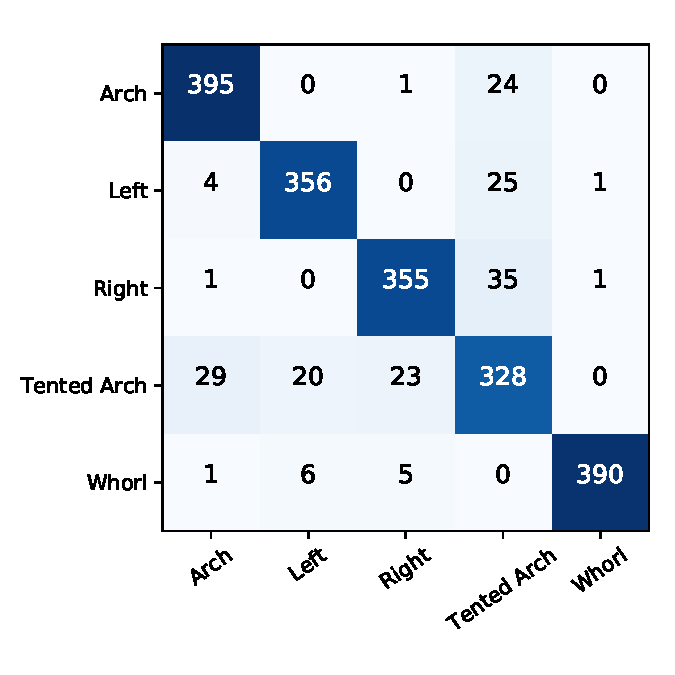
\includegraphics[width=\linewidth]{fig/figs/confusion_matrix_svm_sd4_cross_subject.pdf}
		\caption{SVM -- NIST SD4 }
		\label{fig.cnf_matrix_5class.svm_sd4}
	\end{subfigure}%
	\begin{subfigure}[b]{0.25\textwidth}
		\centering
		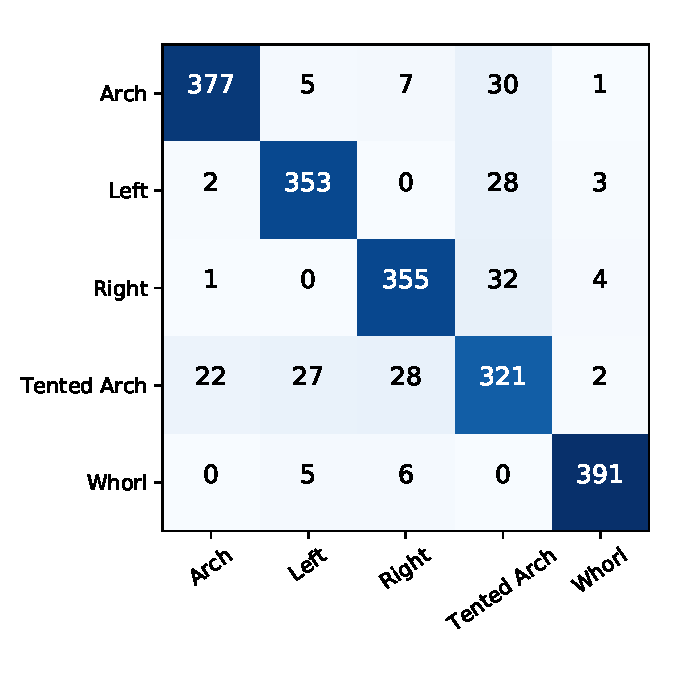
\includegraphics[width=\linewidth]{fig/figs/confusion_matrix_net_sd4_cross_subject.pdf}
		\caption{ConvNet -- NIST SD4 }
		\label{fig.cnf_matrix_5class.net_sd4}
	\end{subfigure}
	\caption{Confusion Matrices for 5-class classification}\label{fig.cnf_matrix_5class}
\end{figure*}

\begin{figure}[!ht]
	\begin{subfigure}[b]{0.25\textwidth}
		\centering
		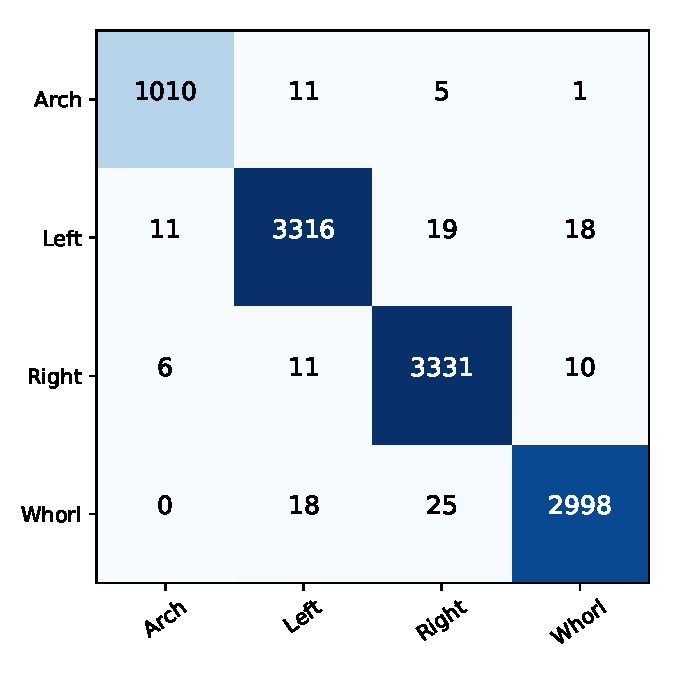
\includegraphics[width=\linewidth]{fig/figs/confusion_matrix_svm_sd14_4class.pdf}
		\caption{SVM -- NIST SD14 }
		\label{fig.cnf_matrix_4class.svm_sd14}
	\end{subfigure}%
	\begin{subfigure}[b]{0.25\textwidth}
		\centering
		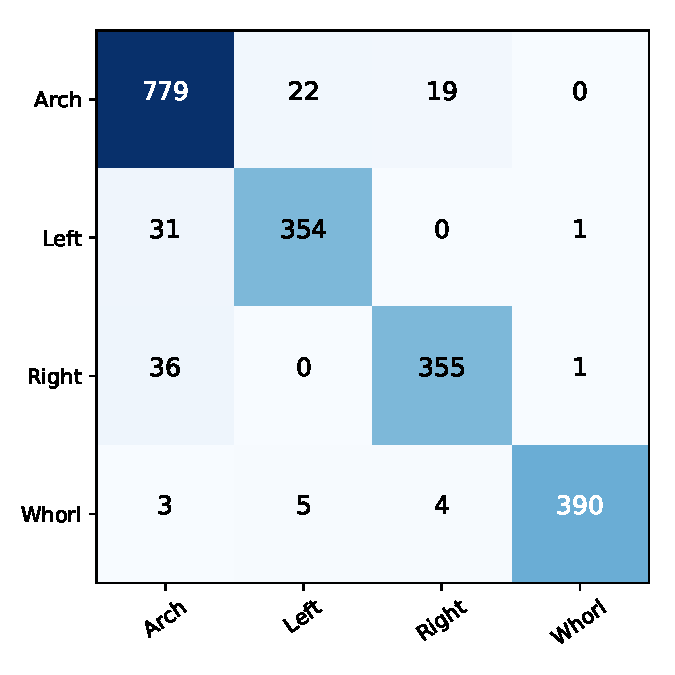
\includegraphics[width=\linewidth]{fig/figs/confusion_matrix_svm_sd4_4class_cross_subject.pdf}
		\caption{SVM -- NIST SD4}
		\label{fig.cnf_matrix_4class.svm_sd4}
	\end{subfigure}%

	\caption{Confusion Matrices for 4-class classification}\label{fig.cnf_matrix_4class}
\end{figure}

%-----------------------------
\subsection{NIST SD14 results}
\label{sec_sd14}

 Table\ref{tab.SD14_result} summarizes our results for NIST SD14 images.
%
ConvNet and SVM achieve similar accuracy ($0.9861$) for 5-class pattern type classification. 
%
However, ConvNet seems to perform slightly better in terms of average precision, recall rate and F1 score.
%
Performance of the SVM classifier is slightly improved when arch and tented arch are combined into one class (4-class classification), achieving accuracy of $0.9875$.
%
The confusion matrices for the 5-class classification are shown in Figures \ref{fig.cnf_matrix_5class.svm_sd14} and \ref{fig.cnf_matrix_5class.net_sd14}.
Figure \ref{fig.cnf_matrix_4class.svm_sd14} shows similar results for the 4-class classification.
%
Despite the unbalanced distribution of fingerprint pattern class types, as indicated by the small number of images of arch and tented arch pattern type compared to other pattern classes, our approach achieves high accuracy.
%
The lowest precision (0.959) and recall (0.950) rates are observed for tented arch.  We believe this is due to lack of sufficient training samples as well as possible label ambiguity.
%
Figure \ref{fig.cnf_matrix_4class.svm_sd14} shows improved precision and recall rates ($0.98$), suggesting combing arch and tented arch classes can eliminate some cases of mis-classifications.

\begin{table}[!ht]
	
	\centering
	\caption{ Experiment results for NIST SD14. Columns 4, 5 and 6 report the average precision, recall and F1 score for all predicted classes. }
	\label{tab.SD14_result}
	\scalebox{0.87}{
	\begin{tabular}{|c|c|c|c|c|c|}
		\hline
		\textbf{method} & \textbf{\begin{tabular}[c]{@{}c@{}}\# of \\ classes\end{tabular}} & \textbf{accuracy} & \textbf{\begin{tabular}[c]{@{}c@{}}average \\ precision\end{tabular}} & \textbf{\begin{tabular}[c]{@{}c@{}}average\\  recall\end{tabular}} & \textbf{\begin{tabular}[c]{@{}c@{}}average \\ F1 score\end{tabular}} \\ \hline
		ConvNet & 5 & 0.9861 & 0.9843 & 0.9793 & 0.9817 \\ \hline
		SVM & 5 & 0.9861 & 0.9822 & 0.9781 & 0.9801 \\ \hline
		SVM & 4 & 0.9875 & 0.9869 & 0.9867 & 0.9868 \\ \hline
	\end{tabular}
}
\end{table}

Figure\ref{fig.fails} shows some examples of mis-classification cases for the NIST SD14.
%

\begin{figure*}[!ht]
	\begin{center}
		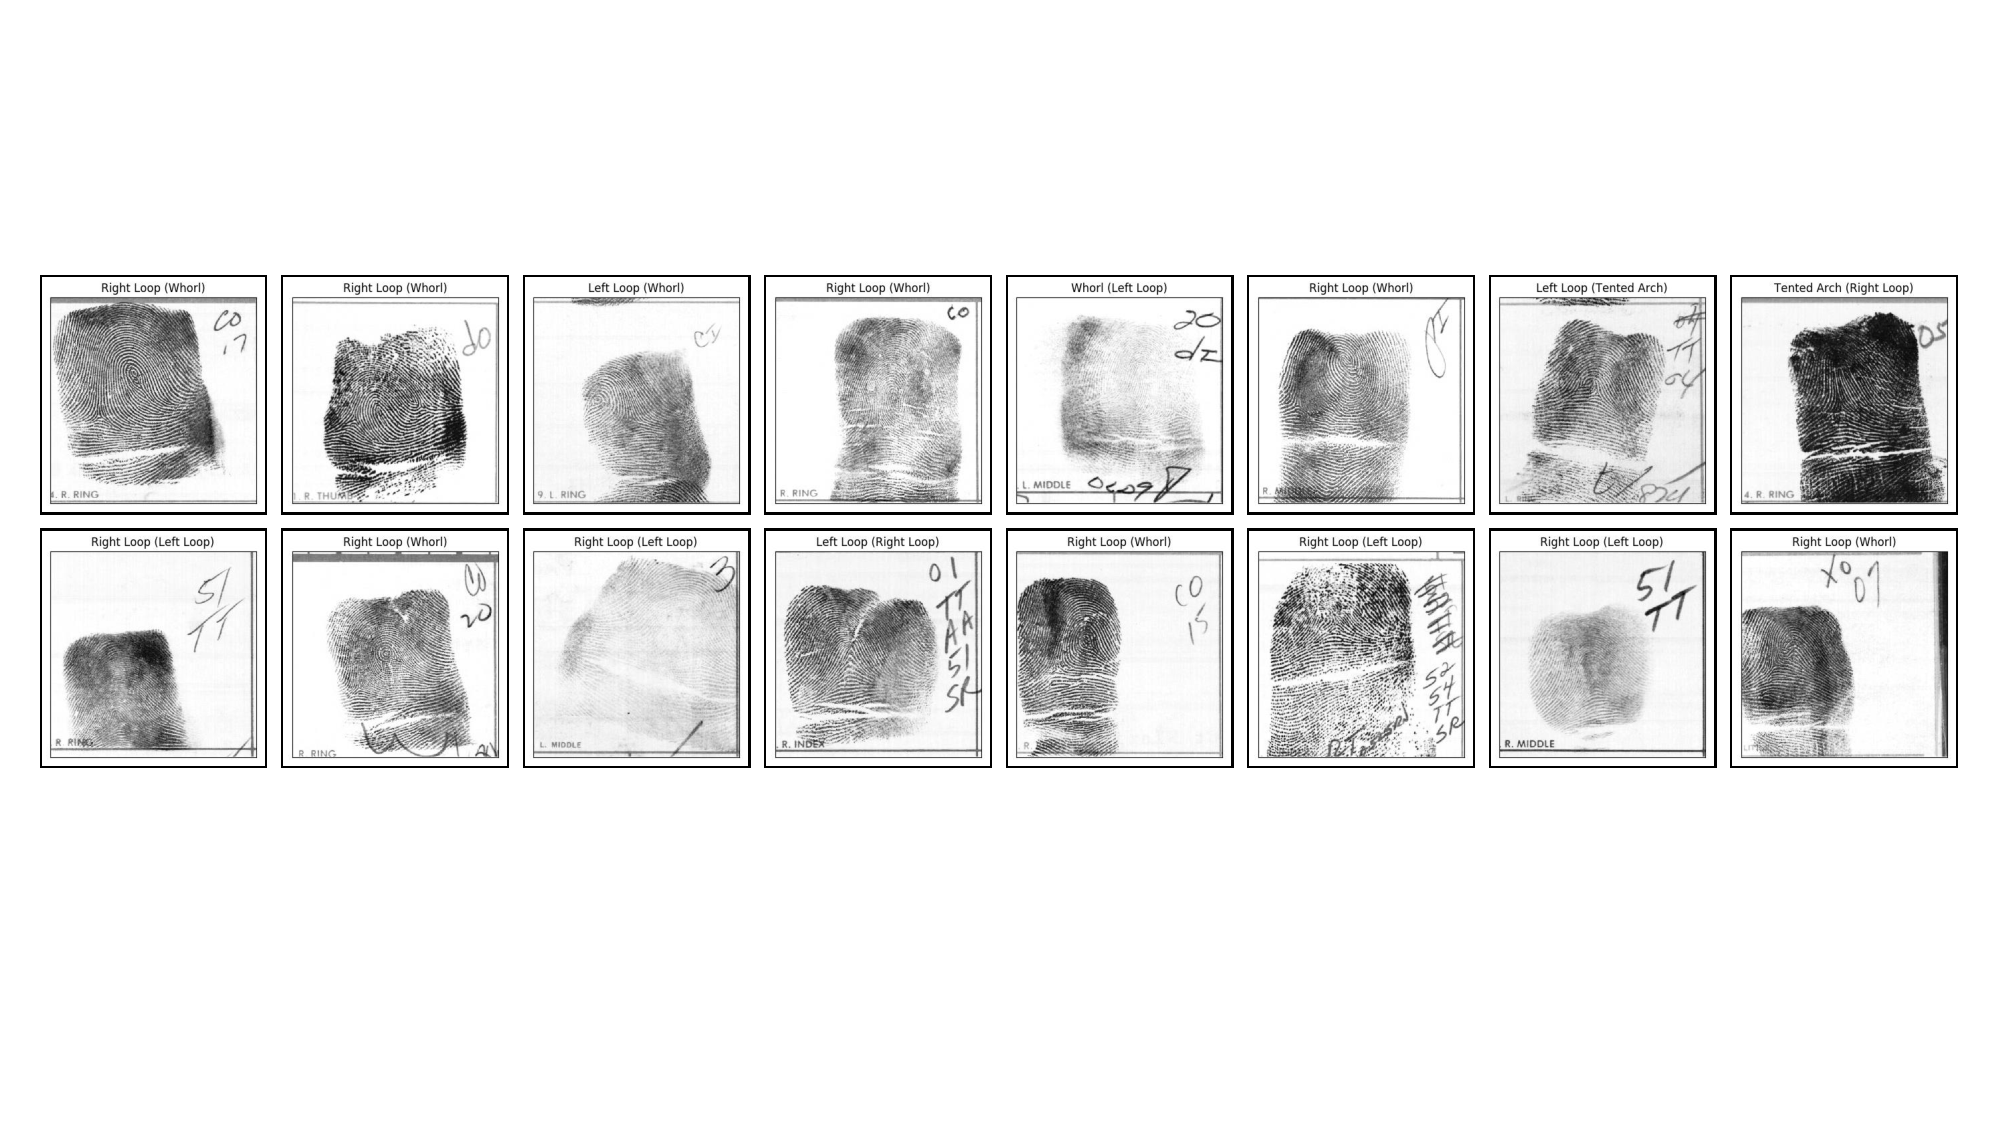
\includegraphics[scale=0.53,clip=true,trim = 5mm 60mm 5mm 45mm]{fig/figs/fail.pdf}
	\end{center}
	\caption{Examples of mis-classification cases for NIST SD14. Each example is labeled with \textit{Prediction}(\textit{Ground Truth})} 
	\label{fig.fails}
\end{figure*}
%----------------------------
\subsection{NIST SD4 Result}
\label{sec_sd4}
 Table\ref{tab.SD4_result} summarizes our results for NIST SD4 images.
%
We make three observations from Table\ref{tab.SD4_result}.
%
First, for both protocols, the SVM performs better than ConvNet not only in accuracy but also in average precision, recall rate and F1 score. 
%
In cross-sample protocol, the accuracy of 5-class SVM is $0.9275$, which is $0.006$ higher than 5-class ConvNet. In cross-finger protocol, the accuracy of 5-class SVM is $0.912$, $0.014$ higher than 5-class ConvNet.
%
Our second observation is that cross-finger protocol shows lower performance compared to cross-sample. For 5-class ConvNet, the accuracy drops $0.023$. SVM shows smaller performance drops: for 5-class SVM, the accuracy is $0.015$ lower, and for 4-class SVM, the accuracy drops $0.011$. 
%
%SVM suffers the smaller performance drop than ConvNet if cross-finger protocol is used.
%
The performance drop is small though, indicating the generalization ability of our proposed method.
%
Thirdly, as we observed and discussed with NIST SD 14 results, the accuracy is improved when tented arch and arch classes are combined into one-class. The accuracy of 4-class SVM is $0.022$ higher than 5-class SVM in cross-sample and $0.027$ higher in cross-finger. This indicates some mis-classification errors can be eliminated by combing arch and tented arch classes.

Figure\ref{fig.cnf_matrix_5class.svm_sd4} and Figure\ref{fig.cnf_matrix_5class.net_sd4} show confusion matrices for 5-class classification using cross-finger protocol. Figure \ref{fig.cnf_matrix_4class.svm_sd4} shows similar results for 4-class classification and cross-finger protocol.
%
Similar to NIST SD 14 results, tented arch gives the lowest precision ($91.8\%$) and lowest precision rate ($94.0\%$) among five classes. 
%
About $17\%$ of the NIST SD 4 images have two class labels.  Because of the ambiguity in class types, the images were assigned  primary and secondary pattern class types. Previous work used performance criteria such that classification into either primary or secondary class being counted as a correct classification. We followed similar performance criteria.
%
%In later experiments, we can see that the mis-labeled samples are ambiguous can be eliminated by introducing the second labels.
%
%For the NIST SD4, about $17\%$ of the samples are ambiguous and are labeled with two classes. Many existing works report their best performance based on these additional labels.
%
%We also evaluate our approach using the additional $17\%$ two labels to compare with other methods and the results are reported in Table.\ref{tab.SD4_result_two_labels}. 
%
The training procedure remains the same as before where we use only the primary pattern class labels for training. 
%
In testing stage, for the $17\%$ of the samples with more than one class label, as long as the prediction matches one of the labels the test sample is considered as a correct classification.  Results tabulated in Table\ref{tab.SD4_result_two_labels} shows a significant performance gain. 
Our proposed ConvNet achieves 0.9535 accuracy for cross-sample protocol, which is 0.032 higher than before.  And 0.945 accuracy, for cross-finger protocol, which is 0.046 higher than before.
%
The proposed 5-class and 4-class SVMs achieve 100\% accuracy for both cross-finger and cross-sample protocols.
%

%
%The proposed 5-class and 4-class SVMs still achieve 1.0 accuracy in this protocol.


\begin{table}[!ht]
	\centering
	\caption{ Experiment results for NIST SD4. Columns 4, 5 and 6 report the average precision, recall and F1 score for all predicted classes. }
	\label{tab.SD4_result}
		\scalebox{0.87}{
	\begin{tabular}{|c|c|c|c|c|c|}
		\hline
		 \textbf{method} & \textbf{\begin{tabular}[c]{@{}c@{}}\# of \\ classes\end{tabular}} & \textbf{accuracy} & \textbf{\begin{tabular}[c]{@{}c@{}}average \\ precision\end{tabular}} & \textbf{\begin{tabular}[c]{@{}c@{}}average\\  recall\end{tabular}} & \textbf{\begin{tabular}[c]{@{}c@{}}average \\ F1 score\end{tabular}} \\ \hline
		 \multicolumn{6}{|c|}{\textbf{Cross-Sample}}      \\ \hline
		ConvNet & 5 & 0.9215 & 0.9225 & 0.9215 & 0.9217 \\ \hline
		SVM & 5 & 0.9275 & 0.9325 & 0.9275 & 0.9288 \\ \hline
		SVM & 4 & 0.9495 & 0.9576 & 0.9459 & 0.9514 \\ 
\hhline{|======|}
\multicolumn{6}{|c|}{\textbf{Cross-Finger}}      \\ \hline
		ConvNet & 5 & 0.8985 & 0.8991 & 0.8986 & 0.8987 \\ \hline
SVM & 5 & 0.9120 & 0.9132 & 0.9117 & 0.9123 \\ \hline
SVM & 4 & 0.9390 & 0.9452 & 0.9357 & 0.9403 \\ \hline
		
\end{tabular}}
\end{table}


\begin{table}[!ht]
	\centering
	\caption{Experiment results for NIST SD4 with two labels.}
	\label{tab.SD4_result_two_labels}
	\begin{tabular}{|c|c|c|c|}
		\hline
		\textbf{method} & \textbf{\# of classes} & \textbf{accuracy} & \textbf{protocol} \\ \hline
		ConvNet & 5 & 0.9535 & cross-sample \\ \hline
		SVM & 5 & 1.0 & cross-sample \\ \hline
		SVM & 4 & 1.0 & cross-sample \\ \hline
		\cite{cao2013fingerprint} & 5 & 0.959 & cross-sample \\ \hline
		\cite{cao2013fingerprint}& 4 & 0.972 & cross-sample \\ \hline
		\cite{wang2014fingerprint} & 4 & 0.980 & not-specified \\ \hline
		ConvNet & 5 & 0.945 & cross-finger \\ \hline
		SVM & 5 & 1.0 & cross-finger \\ \hline
		SVM & 4 & 1.0 & cross-finger \\ \hline
	\end{tabular}
\end{table}

%----------------------------
\subsection{Discussion}
\label{sec_discussion}
%
Experiment results indicate that our proposed method can successfully perform fingerprint pattern class type classification on raw fingerprint images without any feature extraction, and, to the best of our knowledge, achieves better results than previously reported work. 
Using Deep ConvNet as a feature extractor and train a SVM on top of the ConvNet can bring further performance gain compared to a standalone Deep ConvNet.  
%
%Our proposed approach achieves the highest classification accuracy on both NIST SD14 and NIST 4 dataset to the best of our knowledge. 
%
%
Tented arch and arch pattern class types contribute the most error rate among the five classes.  Combining arch and tented arch classes into one improves performance. Allowing more than one class assignment for the ambiguous cases result in further improvements.
%
%Many mis-classified labels can be corrected by combining tented Arch and Arch classes into one class or using additional labels.
%


